\documentclass[a4paper, 12pt]{article}
\usepackage{fontspec} 
\usepackage[utf8]{inputenc}
\usepackage[russian,english]{babel}
\setmainfont{Times New Roman}
\renewcommand{\baselinestretch}{1.5} 


 % для компиляции теперь нужно использовать XeLaTex 
\usepackage{amsfonts}
\usepackage[paper=a4paper,top=13.5mm, bottom=13.5mm,left=20mm,right=20mm,includefoot]{geometry}
\usepackage{indentfirst}
\usepackage{dsfont}
\usepackage{graphicx} 
\graphicspath{{images/}} 
\setlength\fboxsep{3pt} 
\setlength\fboxrule{1pt} 
\usepackage{wrapfig} 
\usepackage{amsmath}
\usepackage{amsthm}
\renewcommand{\proofname}{Доказательство}

\DeclareMathOperator*{\argmin}{arg\,min}
\newcommand{\inde}{\perp\!\!\!\perp}


\theoremstyle{definition}
\newtheorem{definition}{Определение}[section]


\theoremstyle{plain}
\newtheorem{lemma}{Лемма}[section]
\newtheorem{svoistvo}{Свойство}[section]
\newtheorem{theorem}{Теорема}[section]


\title{Исследовательский проект по инстуциональной экономике}
\date{\today}

\begin{document}
\maketitle

\noindent{\bf Аннотация }-- ...

\section{Введение}
Мы устверждаем, что в существуют рынки на которых присутствует сразу несколько игроков со стороны спроса на труд в одном регионе. 
\section{Обзор литературы}

Обозреть статью с моделью по монопсонии. 
Обозреть стаью по олигпсонии, там сделать акцент на том, что олигпосния может многие аномалии объяснить. (Возможно нужно будет также сделать акцент на взаимодействии )
Обозреть эконометрическую статью


\section{Модель}

Многие статьи рассматривают академический рынок труда  как монопсонию (ссылки на статьи). Мы утверждаем, что существуют также рынки олигопсонического типа и совсем не очевидно, что на них будет наблюдаться тенденция к понижению зароботной платы.  Мы рассмотрим модель олигпсонического рынка труда в рамках которой у профессора будет выбор либо остаться в своем регионе и пойти в один из университетов, либо уехать, но понести издержки переезда. Модель будет строится на основе модели монопсонического рынка из статьи Seniority and Monopsony in the Academic Labor Market
Michael R. Ransom (1993). Из неё мы возьмём ...  

Пусть существует рынок в рамках одного города, где присутствует $n$ университетов, предъявляющие спрос на одних и тех же академических работников. Обычно в США в одном городе находится лишь несколько ВУЗов, которые могли бы предъявлять спрос и на одну и ту же рабочую силу, но для общности мы пока буем предполагать, что их $n$. Рынок академических работников основан в своем большинстве на личном взаимодействии, так как преподаватели являются единственными экземплярами предлагающие именно такую комбинацию способностей. Это сильно отличает академический рынок труда от многих других (неплохо бы ссылку). В следствии этого, каждый университет выбирает какую зарплату предложить отдельно для каждого работника. Зарплату предложенную $i$ университетом мы будет обозначать $w_i$. Также будет существовать рыночная заралата $w_m$, именно с такой зарплатой университету придется нанять работника, если профессор, которому предложили зарплату $w_i$ откажется. Университет минимизирует свои ожидаемые издержки: 
\[
EC(w_i) = p_i(w_m, w_i, m, w_{j \neq i})w_i + (1 - p_i(w_m, w_i, m, w_{j \neq i}))w_m
\]

Как мы видим, в зависимости от предложенной зарплаты, зарплаты предложенной другими университетами, зарплаты по рынку и издержкам переезда будет устанавливаться некоторое распределение, случайным исходом для которой будет являться выбор, который сделает преподаватель. Как и в модели с монопсонией мы будем предлагать для простоты, что агенты обладают полной информацией, и единственный источник случайности заключается в выборе профессора одного из университетов. Мы можем предложить, что функция $p_i ( w_m, w_i, m, w_{j \neq i}) $ имеет следующий вид: 
\[
p_i( w_m, w_i, m, w_{j \neq i}) = \frac{p_i(w_i - w_m + \delta m) w_i}{\#\{w_j : w_i = w_j\}}\mathds{1} \{ w_i \geq w_ {i \neq j}\}
\]
Профессор сравнивает предложенную ему зарплату некоторым университетом с зарплатой рынка и своими дисконтированными издержками. Более того, в виду наличия функции индикатора максимальной цены, преподаватель будет рассматривать лишь тот университет, который предложил ему наибольшую зарплату. Всем остальным вузов придется нанимать преподавателя на общем рынке. В виду присутствия ненаблюдаемых факторов решение всё равно остается случайным. 

Возможен также случай, когда несколько университетов предложат максимальную зарплату. Именно этот фактор учитывает знаменатель дроби, который означает, что вероятность попасть в конкретный ВУЗ делится на количество ВУЗов предложивших такую же зарплату. 

Проанализируем поведение стороны спроса на рынке. В статье Olygopsony and Monopsonistic Competition in Labor Markets Bhaskar, A. Manning, Ted To (2002)  рассматриваются различные варианты взаимодействия игроков на олигпсоническом рынке.  Мы будем предполагать, что они не вступают в сговор. Мы считаем, что такая предпосылка вполне оправдана, так как профессора являются единичным товаром, в следствии чего доход от его приобретения почти невозможно разделить легальным путем. 

Заметим, что если вуз устанавливает зарплату ниже чем его конкуренты, то он сталкивается с рыночной ценой с вероятностью 1, соответсвенно в симметричном равновесии  вузы должны установить одинаковую зарплату. И должно быть выполнено следующее условие для каждого конкретного учебного заведения
\[
p_i(w_i - w_m + \delta m) w_i + (1 - p_i(w_i - w_m + \delta m))w_m = \frac{p_i(w_i - w_m + \delta m) w_i}{n} + (1 -\frac{ p_i(w_i - w_m + \delta m)}{n})w_m \leq w_m
\]
Это уравнение означает, что конкретному ВУЗу не выгодно повысить зарплату на любую положительную величину, чтобы повысить вероятность прихода к нему профессора, и более того, в равновесии ожидаемые издержки отдельного ВУЗа не должны превышать рыночную цену на учёного, иначе он обязательно переключится на эту альтернативу
Раскрывая скобки мы получаем 
\[
\frac{(n-1)p_i(w_i - w_m + \delta m) w_i}{n} = \frac{(n-1) p_i(w_i - w_m + \delta m) w_m}{n}
\]
\[
w_i = w_m
\]

Мы видим, что в случае такой конкуренции будет установлено равновесие в котором каждый вуз предлагает одинаковую зарплату равную рыночной, ученый в свою очередь с вероятностью $p(\delta m)/n$ выбирает один из вузов, и с вероятностью $1 - p(\delta m)$ уезжает из города. Соответсвенно мы не ожидаем увидеть на данных тенденцию к понижению зарплаты на таких рынках. Более того, можно сказать, что почти не существует ситуаций, когда несколько ВУЗов в одном городе предлагают профессору рыночную зарплату. Но так как теперь ВУЗам безразлично с точки зрения модели, какого профессора брать, то со стороны спроса вполне может остаться только один агент. Также естественно предположить, что не за каждого профессора идёт такая борьба на рынке труда, следовательно на данных мы ожидаем увидеть не противоположный эффект, как в предыдущих статьях, но более слабый. 

Мы выяснили, что в случае такой ситуации на рынке мы не ожидаем понижения зарплат. Аналогично монопсонической модели мы можем предложить, что в течение жизни профессора через равные промежутки времени перед ним встаёт снова выбор, уехать или нет.  Его зарплата в этот момент обновляется в результате реализации случайного события.  Именно на основании такого анализа авторы статьи [1] и пришли к выводу о падении зарплат. В связи с этим мы можем предположить, что конкуренция за профессора не ведется на протяжении всех периодов, что по нашему мнению является вполне осознанной предпосылкой, так как профессора редко меняют университет, исходя из этого можно заключить, что и в конкуренцию за профессоров ВУЗы вступают редко. Следовательно в какие то периоды, мы будем снова оказываться в случае монопсонии. Тогда на протяжении всех периодов зарплата будет вести себя скачкообразно, если профессор всё это время оставался в городе. % если будет не хватать места, то я опишу математически этот эффект

В динамике мы получили, что эффект понижения зарплат на таких рынках будет наблюдаться, только теперь он будет  слабее, чем на рынках, где лишь один университет определенного уровня.

\section{Кейс}

В качестве примера, иллюстрирующего вышеописанную модель, будет рассмотрен Хьюстонская система университетов. Во-первых, университеты внутри этой системы независимы и примерно одного ранга (Tier 2), то есть между ними существует конкуренция за рабочую силу. Во-вторых, в Хьюстоне также присутствует достаточно большое количество университетов второго ранга, например, Техас Саутерн и Университет Конкордия. Все эти учебные заведения расположены в пределах города Хьюстон и его пригорода. Исходя из данной информации можно сделать вывод, что рынок академического труда города Хьюстон можно рассматривать как олигопсонию. Заметим, что это справедливо только для университетов второго ранга и ниже, потому что в данном городе присутствует только один университет первого ранга Райс.

Данные о работниках Хьюстонской системы находятся в открытом доступе на сайте: http://salaries.texastribune.org/university-of-houston/. Перед началом анализа данные были обработаны. Сначала была проведена очистка данных от работников департаментов, занимающихся административной и обслуживающей деятельностями. Далее были оставлены только работники, занимающиеся преподаванием, то есть профессоры. Наконец, была добавлена переменная $seniority$, показывающая сколько полных лет индивид проработал в данном университете.
Для анализа будут использованы следующие переменные из ранее упомянутой базы данных: $rate$ --- уровень заработной платы, $sex$ --- пол индивида (1 --- мужчина), $Fullp$ --- является ли индивид "полным профессором", $Type$ --- полный рабочий день или частичный, $Foreign$ --- показывает расу (0 --- европеоидная, 1 --- остальные).

Дескриптивная статистика выборки:

\begin{center}
\begin{tabular}{|c|c|c|}
\hline 
• & lograte & seniority \\ 
\hline 
Среднее & 11.47 & 13.35 \\ 
\hline 
Медиана & 11.45 & 10.00 \\ 
\hline 
Стандартное отклонение & 0.39 & 12.11 \\ 
\hline 
N=1016 & • & • \\ 
\hline 
\end{tabular} 
\end{center}

\begin{center}
\begin{tabular}{|c|c|c|}
\hline 
• & N & \% \\ 
\hline 
Мужчины & 688 & 67.72 \\ 
\hline 
"Полные" профессора & 351 & 34.55 \\ 
\hline 
Работающие полный день & 994 & 97.83 \\ 
\hline 
"Европейцы" & 634 & 62.40 \\ 
\hline 
\end{tabular} 
\end{center}

Воспользуемся Минцеровским уравнением для того, чтобы оценить влияние рабочего стажа на заработную плату:

$$lograte=\alpha_1+\alpha_2 Sex+\alpha_3 Seniority +\alpha_4 Fullp+\alpha_5 Type +\alpha_6 Foreign$$

где $lograte$ --- логарифм заработной платы.

Значения полученных коэфициентов:

\begin{center}
\begin{tabular}{|c|c|c|}
\hline 
• & Оценка коэфициента & Стандартное отклонение оценки \\ 
\hline 
Свобдный член & 10.79754 & 0.07216 \\ 
\hline 
sex & 0.12098 & 0.02134 \\ 
\hline 
seniority & -0.00588 & 0.00095 \\ 
\hline 
fullp & 0.51297 & 0.02447 \\ 
\hline 
type & 0.48461 & 0.06923 \\ 
\hline 
foreign & 0.07161 & 0.02056 \\ 
\hline 
\end{tabular} 
\end{center}

Все полученные коэфициенты значимы даже при очень маленьких уровнях значимости ($\alpha<0.001$).

В нашем примере $R^2=0.36$. Такое значение позволяет нам думать, что зависимость однозначно существует, но частично остаток должен объясниться с помощью дополнительных регрессоров, например, опыт или возраст и квадрат этих величин. В данном уравнении не было использовано таких переменных, ибо в нашей базе данных не было возраста преподавателей, а восстанавливать его достаточно сложно.
Также коэффициент, который мы получили при seniority больше, чем аналогичный у Ransom 1993. Этот факт можно объяснить как раз из-за потерянных нами важных переменных (в уравнении Минцера возраст является одним из важнейших показателей).

Также, возможные проблемы могут возникать из-за того, что выборка не является репрезентативной. Такой вывод можно сделать исходя из графика плотности логарифма заработной платы: в идеальной ситуации логарифм заработной платы должен быть распределен нормально, однако, в здесь наблюдается смещение в сторону более высоких зарплат профессоров.


\begin{center}
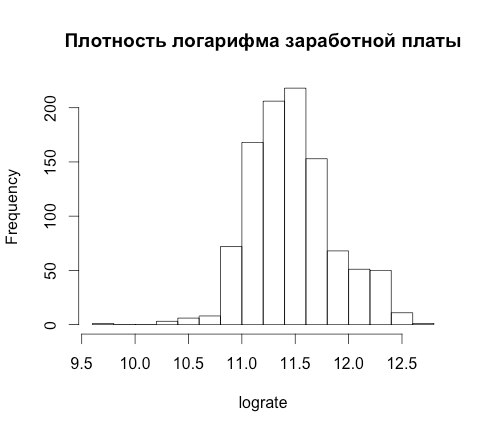
\includegraphics[scale=0.5]{image1}
\end{center}

\section{Заключение}




\end{document}



